\documentclass[12pt,letterpaper]{article}
\usepackage[utf8]{inputenc}
\usepackage[spanish]{babel}
\usepackage{graphicx}
\usepackage[left=2cm,right=2cm,top=2cm,bottom=2cm]{geometry}
\usepackage{graphicx} % figuras
% \usepackage{subfigure} % subfiguras
\usepackage{float} % para usar [H]
\usepackage{amsmath}
%\usepackage{txfonts}
\usepackage{stackrel} 
\usepackage{multirow}
\usepackage{enumerate} % enumerados
\renewcommand{\labelitemi}{$-$}
\renewcommand{\labelitemii}{$\cdot$}
% \author{}
% \title{Caratula}
\begin{document}

% Fancy Header and Footer
% \usepackage{fancyhdr}
% \pagestyle{fancy}
% \cfoot{}
% \rfoot{\thepage}
%

% \usepackage[hidelinks]{hyperref} % CREA HYPERVINCULOS EN INDICE

% \author{}
\title{Caratula}

\begin{titlepage}
\begin{center}
\large{UNIVERSIDAD PRIVADA DE TACNA}\\
\vspace*{-0.025in}
\begin{figure}[htb]
\begin{center}

\includegraphics[width=4cm]{./Imagenes/logo}
\end{center}
\end{figure}
\vspace*{0.15in}
INGENIERIA DE SISTEMAS  \\

\vspace*{0.5in}
\begin{large}
TEMA:\\
\end{large}

\vspace*{0.1in}
\begin{Large}
\textbf{Informe Sesión de Laboratorio Nro 03} \\
\end{Large}

\vspace*{0.3in}
\begin{Large}
\textbf{CURSO:} \\
\end{Large}

\vspace*{0.1in}
\begin{large}
INTELIGENCIA DE NEGOCIOS\\
\end{large}

\vspace*{0.3in}
\begin{Large}
\textbf{DOCENTE(ING):} \\
\end{Large}

\vspace*{0.1in}
\begin{large}
 Patrick Jose Cuadros Quiroga\\
\end{large}

\vspace*{0.2in}
\vspace*{0.1in}
\begin{large}
Integrantes: \\
\begin{flushleft}


Zuñiga Silva, Roby Gerson  	           \hfill	(2015052684) \\


\end{flushleft}
\end{large}
\end{center}

\end{titlepage}

\section{Informe Creando un Reporte Interactivo en Power BI} 
\begin{flushleft}


\begin{itemize}
\textbf{Ejercicio 1: Conectando a Power BI a datos}\\
\textbf{ }\\
\textbf{Tarea 1: }Conectar a datos existentes \\
\textbf{ }\\

1. Abrir SQL Server Management Studio, y conectar a la instancia de base de datos (local) utilizando
autenticación de Windows.\\
2. En el menú Archivo (File), en el submenu Abrir (Open), hacer click en Project/Solution, y buscar el archivo
Project.ssmssln.\\
\textbf{ }\\
\begin{center}
	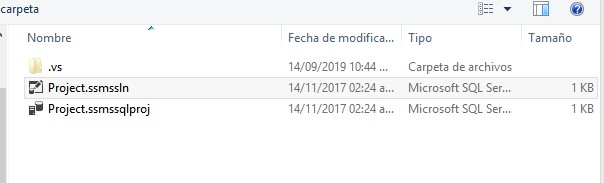
\includegraphics[width=15cm]{./Imagenes/image1} 
	\end{center}
\textbf{ }\\


3. En el Explorador de Soluciones, expandir Consultas (Queries), y luego hacer doble click en el archivo Lab
Exercise 1.sql.\\
\textbf{ }\\
\begin{center}
	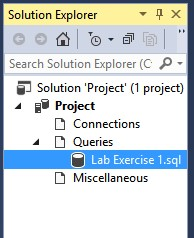
\includegraphics[width=5cm]{./Imagenes/image2} 
	\end{center}
\textbf{ }\\
\textbf{ }\\
\textbf{ }\\
\textbf{ }\\
\textbf{ }\\
\textbf{ }\\
\textbf{ }\\
\textbf{ }\\
\textbf{ }\\
\textbf{ }\\
4. Abrir Power BI Desktop.\\
5. En la ventana Power BI Desktop, hacer click en Obtener Data (Get Data).\\
6. En el cuadro Obtener Datos, click base de datos Microsoft SQL, y entonces click en Conectar\\

\textbf{ }\\
\begin{center}
	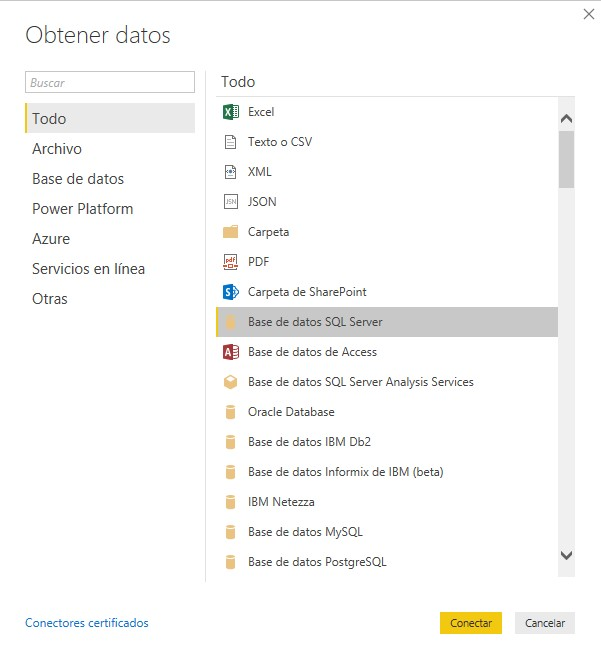
\includegraphics[width=13cm]{./Imagenes/image3} 
	\end{center}
\textbf{ }\\
\textbf{ }\\
\textbf{ }\\
\textbf{ }\\
\textbf{ }\\
\textbf{ }\\
\textbf{ }\\
\textbf{ }\\
\textbf{ }\\
\textbf{ }\\
\textbf{ }\\
\textbf{ }\\
\textbf{ }\\
\textbf{ }\\
7. En la ventana base de datos Server database, En Servidor, escribir (local).\\
8. En Base de Datos (opcional), tipear AdventureWorksLT.\\
9. Expandir el cuadro Opciones Avanzadas. Copiar el script Task 1 del archivo Lab Exercise 1.sql. y pegar\\
la consulta en Power BI, en el cuadro sentencia SQL. Luego presionar OK.\\
10. En la ventana de vista preliminar click en Cargar.\\
11. En Power BI Desktop, click Obtener Datos y luego click en Mas.\\
\textbf{ }\\
\begin{center}
	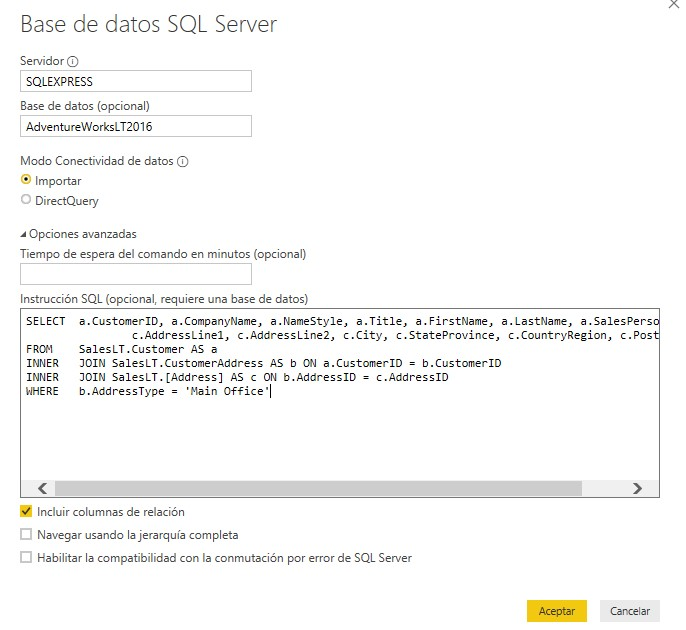
\includegraphics[width=15cm]{./Imagenes/image4} 
	\end{center}
\textbf{ }\\
\begin{center}
	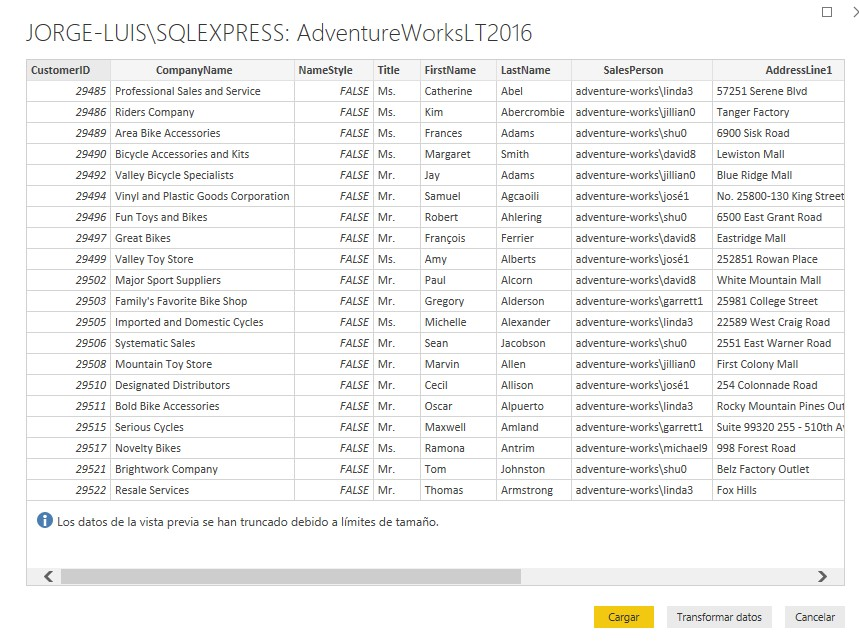
\includegraphics[width=16cm]{./Imagenes/image5} 
	\end{center}
\textbf{ }\\
\textbf{ }\\
\textbf{ }\\
\textbf{ }\\
\textbf{ }\\
\textbf{ }\\
\textbf{ }\\
\textbf{ }\\
\textbf{ }\\
\textbf{ }\\
\textbf{ }\\
\textbf{ }\\
\textbf{ }\\
\textbf{ }\\
\textbf{ }\\
\textbf{ }\\
\textbf{ }\\
\textbf{ }\\
\textbf{ }\\
\textbf{ }\\
\textbf{ }\\
\textbf{ }\\
\textbf{ }\\
\textbf{ }\\
12. Repetir los pasos del 6 al 10, utilizando el script Task 2.\\
13. De regreso en el reporte. Guardar el archivo como AdventureWorksLT Sales.pbix\\
\textbf{ }\\
\begin{center}
	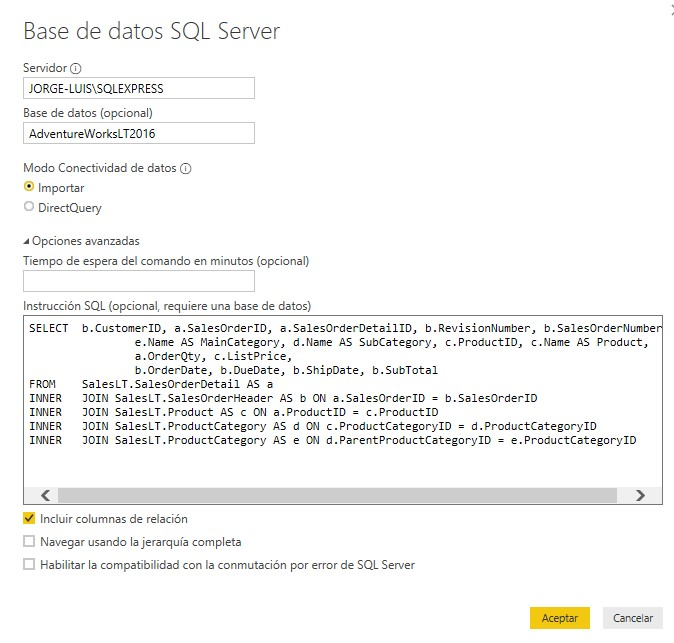
\includegraphics[width=12cm]{./Imagenes/image6} 
	\end{center}
\textbf{ }\\
\textbf{ }\\
\begin{center}
	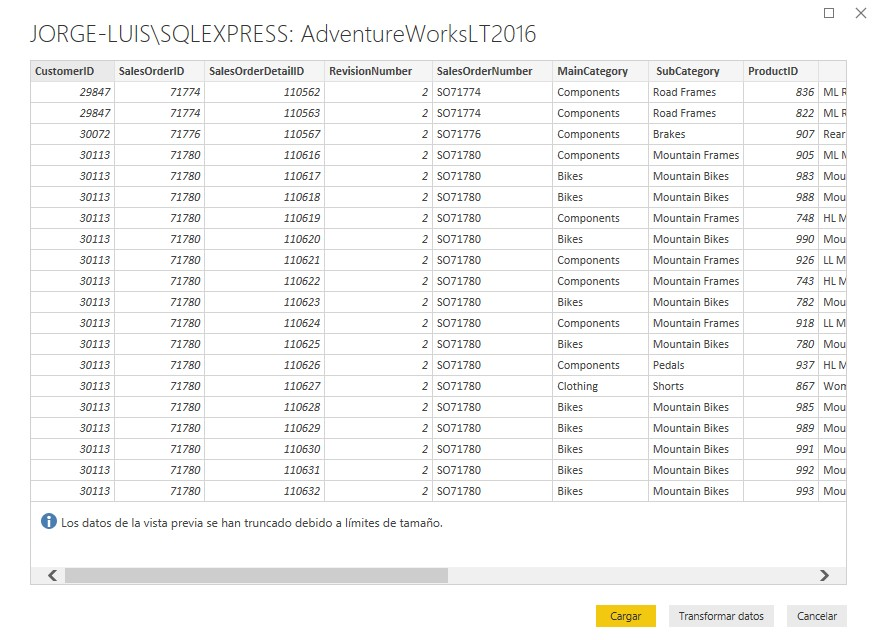
\includegraphics[width=12cm]{./Imagenes/image7} 
	\end{center}
\textbf{ }\\

\textbf{ }\\
\textbf{Tarea 2: }Graficar Datos  \\
\textbf{ }\\

1. En el panel Campos (Fields), click derecho sobre Query1, Renombrar, tipear Customers y presionar Enter.\\
2. Para el Query2, hacer lo mismo del paso 1 y colocar el nombre Sales.\\
3. Expandir ambas tablas para ver todas las filas.\\
\textbf{ }\\
\begin{center}
	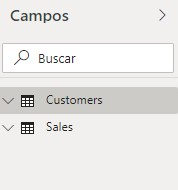
\includegraphics[width=4cm]{./Imagenes/image8} 
	\end{center}
\textbf{ }\\
4. En la barra de navegación izquierda, haga clic en Datos.\\
5. En el panel Campos, haga clic en la tabla Clientes, si aún no está seleccionada.\\
6. Haga clic con el botón derecho en la columna NameStyle y haga clic en Eliminar.\\
7. En el cuadro de diálogo Eliminar columna, haga clic en Eliminar.\\

\textbf{ }\\
\begin{center}
	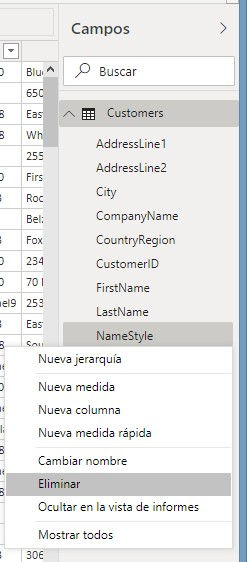
\includegraphics[width=4cm]{./Imagenes/image9} 
	\end{center}
\textbf{ }\\


\textbf{ }\\
\textbf{ }\\
\textbf{ }\\
\textbf{ }\\
\textbf{ }\\
\textbf{ }\\
8. Repetir el paso 6 y 7 para la columna SalesPerson\\
\textbf{ }\\
\begin{center}
	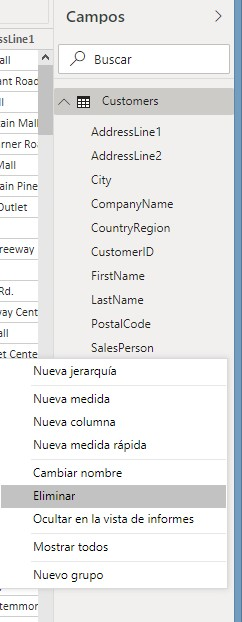
\includegraphics[width=4cm]{./Imagenes/image10} 
	\end{center}
\textbf{ }\\

9. Haga clic con el botón derecho en la columna CustomerID y luego haga clic en Ocultar en vista de informe.\\
\textbf{ }\\
\begin{center}
	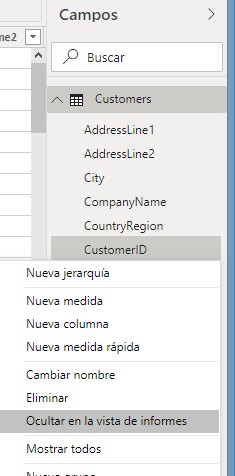
\includegraphics[width=4cm]{./Imagenes/image11} 
	\end{center}
\textbf{ }\\
\textbf{ }\\
\textbf{ }\\
\textbf{ }\\
10. Haga clic en el encabezado de la columna AddressLine1.\\
\textbf{ }\\
\begin{center}
	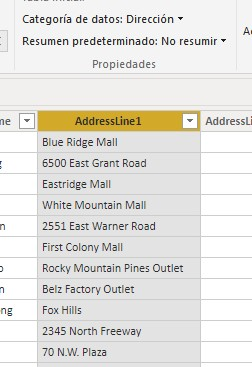
\includegraphics[width=6cm]{./Imagenes/image12} 
	\end{center}
\textbf{ }\\
11. En la cinta de Modelado, en el grupo Propiedades, haga clic en Categoría de datos: Sin clasificar y luego haga clic en
Habla a.\\
12. Haga clic en el encabezado de la columna Ciudad.\\
13. En la cinta de Modelado, en el grupo Propiedades, haga clic en Categoría de datos: Sin clasificar y luego en Ciudad.\\
14. Haga clic en el encabezado de columna StateProvince.\\
15. En la cinta de Modelado, en el grupo Propiedades, haga clic en Categoría de datos: Sin clasificar y luego haga clic en Estado o
Provincia.\\
\textbf{ }\\
\begin{center}
	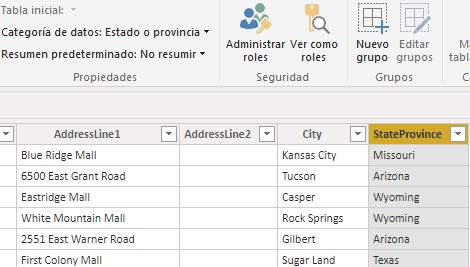
\includegraphics[width=6cm]{./Imagenes/image13} 
	\end{center}
\textbf{ }\\
\textbf{ }\\
\begin{center}
	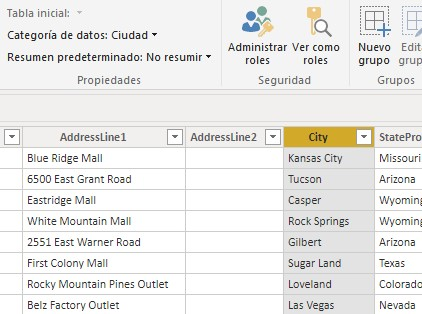
\includegraphics[width=6cm]{./Imagenes/image14} 
	\end{center}
\textbf{ }\\

16. Haga clic en el encabezado de columna CountryRegion.\\
17. En la cinta de Modelado, en el grupo Propiedades, haga clic en Categoría de datos: Sin clasificar y luego haga clic en
País / Región\\
\textbf{ }\\
\begin{center}
	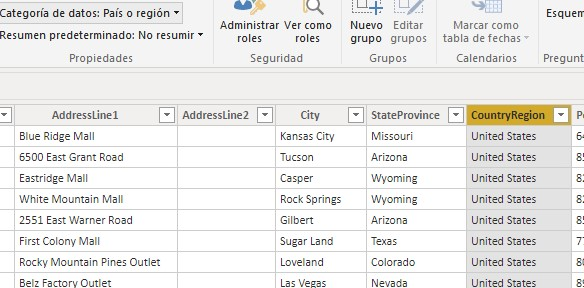
\includegraphics[width=8cm]{./Imagenes/image15} 
	\end{center}
\textbf{ }\\

18. Haga clic en el encabezado de columna Código postal.\\
19. En la cinta de Modelado, en el grupo Propiedades, haga clic en Categoría de datos: Sin clasificar y luego haga clic en Postal
Código.\\
\textbf{ }\\
\begin{center}
	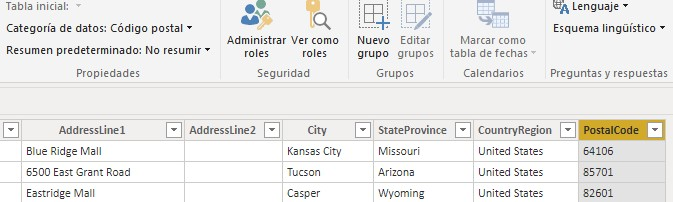
\includegraphics[width=8cm]{./Imagenes/image16} 
	\end{center}
\textbf{ }\\

20. En la cinta de Modelado, en el grupo Cálculos, haga clic en Nueva columna y luego en la barra de fórmulas, escriba
siguiente expresión y presione Entrar:\\ FullAddress = Customers[AddressLine1] \& ", " \& Customers[City] \& ", " \&
Customers[StateProvince] \& ", "\& Customers[CountryRegion] \& ", " \&
Customers[PostalCode]\\
\textbf{ }\\
\begin{center}
	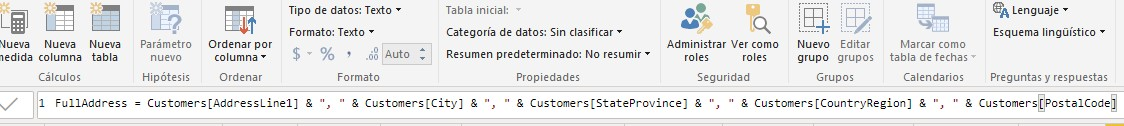
\includegraphics[width=16cm]{./Imagenes/image17} 
	\end{center}
\textbf{ }\\

21. En el panel Campos, haga clic en Ventas.\\
22. Haga clic con el botón derecho en la columna RevisionNumber y haga clic en Eliminar.\\
\textbf{ }\\
\begin{center}
	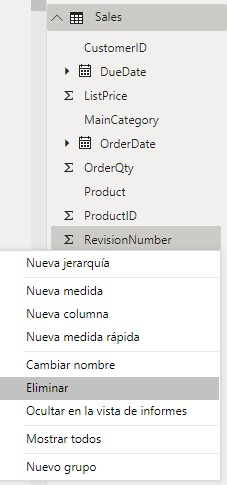
\includegraphics[width=6cm]{./Imagenes/image18} 
	\end{center}
\textbf{ }\\

23. En el cuadro de diálogo Eliminar columna, haga clic en Eliminar.\\
24. Realice el paso 23 y 34 para la columna SalesOrderNumber.\\
\textbf{ }\\
\begin{center}
	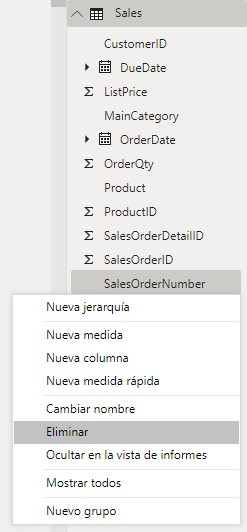
\includegraphics[width=6cm]{./Imagenes/image19} 
	\end{center}
\textbf{ }\\

25. Haga clic con el botón derecho en la columna CustomerID y luego haga clic en Ocultar en vista de informe.\\
\textbf{ }\\
\begin{center}
	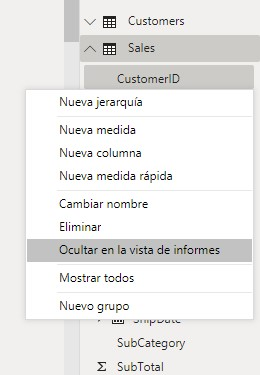
\includegraphics[width=6cm]{./Imagenes/image20} 
	\end{center}
\textbf{ }\\

26. Realice el paso 26 para las columnas SalesOrderID y SalesOrderDetailID.\\

\textbf{ }\\
\begin{center}
	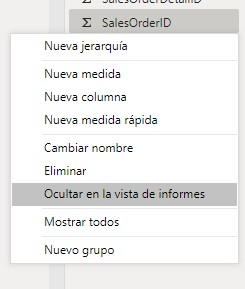
\includegraphics[width=6cm]{./Imagenes/image21} 
	\end{center}
\textbf{ }\\
\textbf{ }\\
\begin{center}
	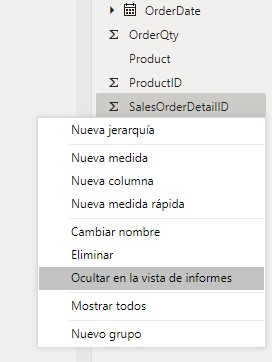
\includegraphics[width=6cm]{./Imagenes/image22} 
	\end{center}
\textbf{ }\\

\textbf{ }\\
\textbf{ }\\
\textbf{ }\\
\textbf{ }\\
\textbf{ }\\
\textbf{ }\\
\textbf{ }\\
\textbf{ }\\
\textbf{ }\\
\textbf{ }\\
\textbf{ }\\

27. En la cinta de Modelado, en el grupo Cálculos, haga clic en Nueva columna y luego en la barra de fórmulas, escriba
siguiente expresión y presione Entrar: LineTotal = Sales[OrderQty] * Sales[ListPrice]\\
\textbf{ }\\
\begin{center}
	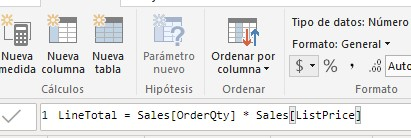
\includegraphics[width=16cm]{./Imagenes/image23} 
	\end{center}
\textbf{ }\\

28. Haga clic en el encabezado de la columna LineTotal.\\
29. En la cinta de Modelado, en el grupo Formato, haga clic en Formato: General, seleccione Moneda y luego haga clic en \$
Inglés Estados Unidos).\\
\textbf{ }\\
\begin{center}
	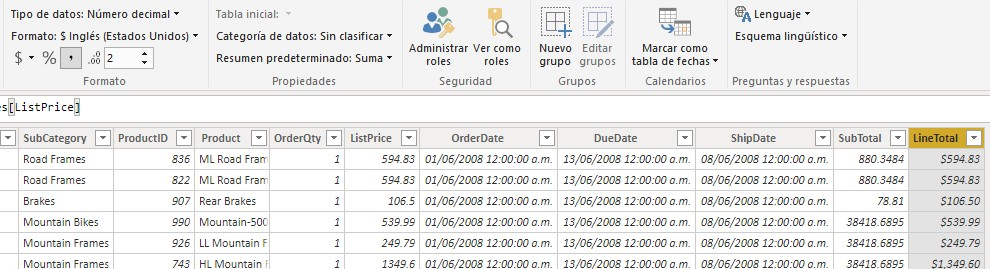
\includegraphics[width=16cm]{./Imagenes/image24} 
	\end{center}
\textbf{ }\\

30. En la cinta de Modelado, en el grupo Cálculos, haga clic en Nueva medida, y luego en la barra de fórmulas, escriba
siguiente expresión y presione Entrar:
TargetSales = SUM ('Ventas' [LineTotal]) * 1.2\\
\textbf{ }\\
\begin{center}
	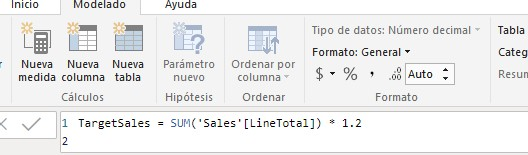
\includegraphics[width=16cm]{./Imagenes/image25} 
	\end{center}
\textbf{ }\\

\textbf{ }\\
\textbf{ }\\
\textbf{ }\\
\textbf{Tarea 3: }Combinar Data  \\
\textbf{ }\\

1. En el Explorador de archivos, y luego abra el archivo States.xlsx.\\
2. En la hoja de trabajo de Estados, seleccione todos los valores en las dos columnas y luego presione Ctrl + C.\\
3. En Power BI Desktop, en la cinta de Inicio, haga clic en Introducir datos.\\


\textbf{ }\\
\textbf{ }\\
\begin{center}
	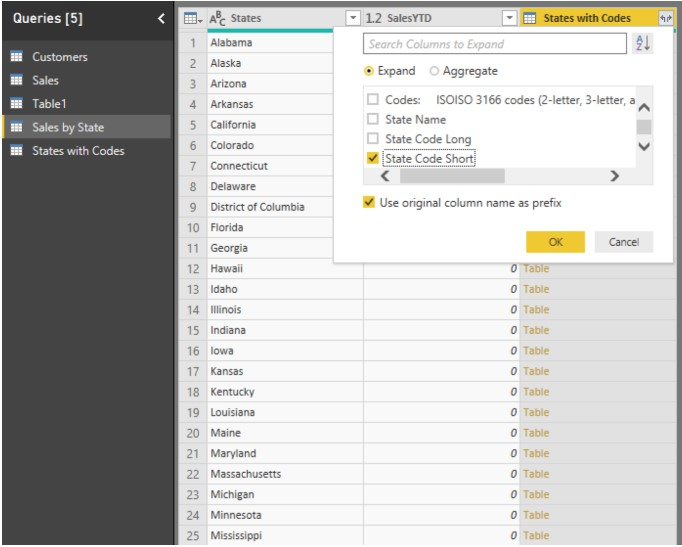
\includegraphics[width=10cm]{./Imagenes/image26} 
	\end{center}
\textbf{ }\\
4. En el cuadro de diálogo Crear tabla, haga clic en la tabla y luego presione Ctrl + V. Power BI detecta que la primera fila es
Un encabezado de columna.\\
5. En el cuadro Nombre, escriba Ventas por estado y luego haga clic en Cargar.\\

\textbf{ }\\
\begin{center}
	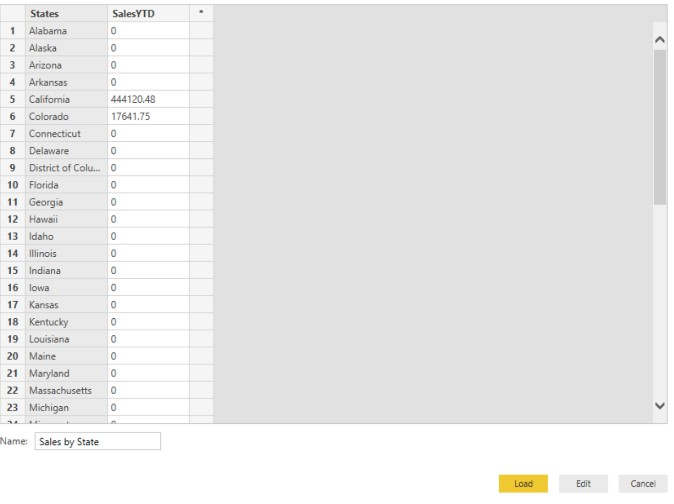
\includegraphics[width=10cm]{./Imagenes/image27} 
	\end{center}
\textbf{ }\\

\textbf{ }\\
\textbf{ }\\
6. En la cinta de Inicio, haga clic en Obtener datos y luego en Web.\\
7. En el cuadro de diálogo De la web, en el cuadro URL, escriba:\\
\begin{center}
	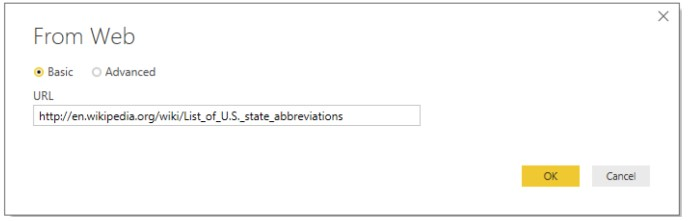
\includegraphics[width=16cm]{./Imagenes/image28} 
	\end{center}
\textbf{ }\\

8. En el cuadro de diálogo Navegador, seleccione Códigos y abreviaturas para estados, territorios y otros Estados Unidos.
regiones, y luego haga clic en Cargar.\\

\textbf{ }\\
\begin{center}
	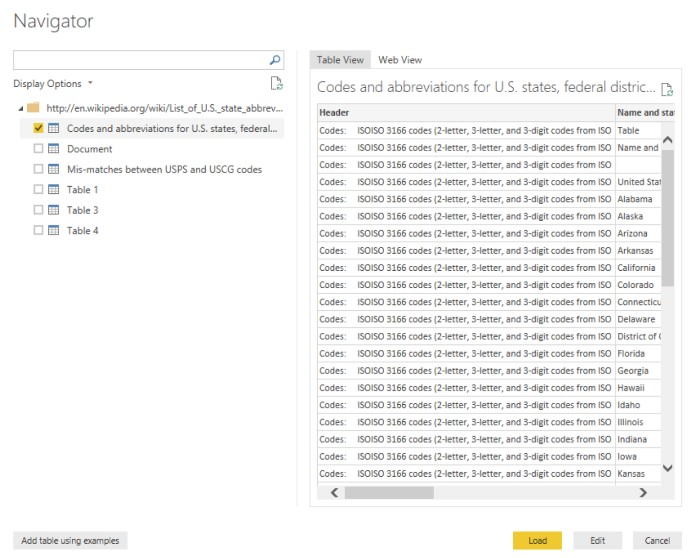
\includegraphics[width=15cm]{./Imagenes/image29} 
	\end{center}
\textbf{ }\\

\textbf{ }\\
\textbf{ }\\
\textbf{ }\\
\textbf{ }\\
\textbf{ }\\
\textbf{ }\\
9. En el panel Campos, haga clic en Códigos y abreviaturas para estados, territorios y otras regiones de EE. UU. Para
Mostrar los datos. La tabla tiene 26 filas en la parte inferior que no son necesarias.\\
10. En la cinta de Inicio, en el grupo Datos externos, haga clic en Editar consultas, luego haga clic en Editar consultas.\\
11. En el Editor de consultas, en el panel Consultas, haga clic en Códigos y abreviaturas para estados, territorios y otros Estados Unidos.\\
regiones.\\
12. En la cinta de Inicio, haga clic en Reducir filas, haga clic en Eliminar filas y luego haga clic en Eliminar filas inferiores.\\
13. En el cuadro de diálogo Eliminar filas inferiores, en el cuadro Número de filas, escriba 26 y luego haga clic en Aceptar.\\
\textbf{ }\\
\begin{center}
	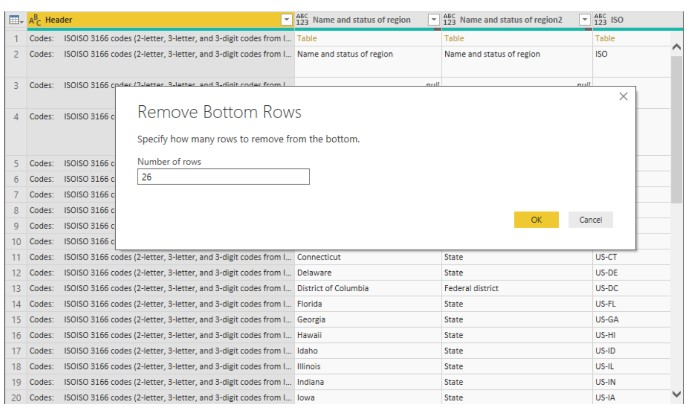
\includegraphics[width=15cm]{./Imagenes/image30} 
	\end{center}
\textbf{ }\\
\textbf{ }\\
\textbf{ }\\
\textbf{ }\\
\textbf{ }\\
\textbf{ }\\
\textbf{ }\\
\textbf{ }\\
\textbf{ }\\
\textbf{ }\\
\textbf{ }\\
\textbf{ }\\
\textbf{ }\\
\textbf{ }\\
\textbf{ }\\
\textbf{ }\\
16. En la cinta de Inicio, haga clic en Administrar columnas, haga clic en Eliminar columnas y luego haga clic en Eliminar columnas.\\
17. En el panel Configuración de consulta, en Propiedades, en el cuadro Nombre, escriba Estados con códigos y luego presione
Entrar.\\
18. En la cinta de Inicio, en el grupo Transformar, haga clic en Usar primera fila como encabezados.\\
19. Haga clic con el botón derecho en el encabezado de la columna de Estados Unidos de América, haga clic en Cambiar nombre, escriba Nombre del estado y, a continuación, presione
Entrar.\\
20. Haga clic con el botón derecho en el encabezado de la columna US USA 840, haga clic en Cambiar nombre, escriba Código de estado largo y luego presione Entrar.\\
21. Haga clic con el botón derecho en el encabezado de la columna de EE. UU., Haga clic en Cambiar nombre, escriba Código de estado corto y luego presione Entrar.\\

\textbf{ }\\
\begin{center}
	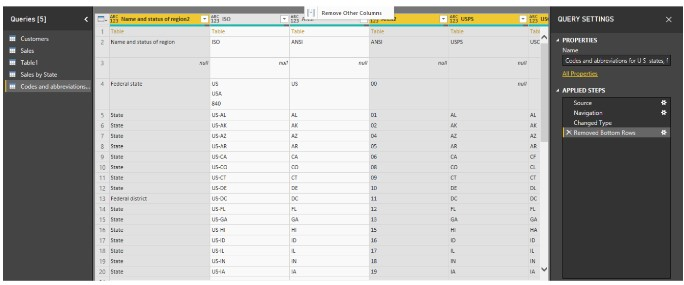
\includegraphics[width=15cm]{./Imagenes/image31} 
	\end{center}
\textbf{ }\\
\textbf{ }\\
\begin{center}
	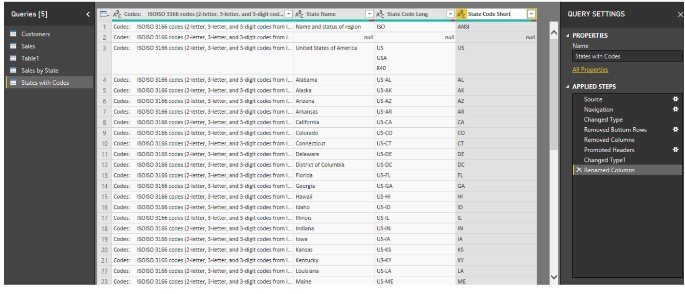
\includegraphics[width=15cm]{./Imagenes/image32} 
	\end{center}
\textbf{ }\\
\textbf{ }\\
\textbf{ }\\
\textbf{ }\\
\textbf{ }\\
\textbf{ }\\
22. En el panel Consultas, haga clic en Ventas por estado.\\
23. En la cinta de Inicio, haga clic en Combinar y luego en Combinar consultas.\\
24. En el cuadro de diálogo Fusionar, en la tabla Ventas por estado, haga clic en la columna Estados.\\
25. En la lista, haga clic en Estados con códigos, haga clic en la columna Nombre del estado y luego haga clic en Aceptar. La nueva columna es
agregado a la tabla y contiene la tabla Estados combinados con códigos.\\
26. En el encabezado de la columna, haga clic en el icono Expandir, desactive (Seleccionar todas las columnas), seleccione Código de estado corto,
y luego haga clic en Aceptar. La columna ahora muestra solo los códigos de estado.\\
27. Haga clic con el botón derecho en la columna, haga clic en Cambiar nombre, escriba Código de estado y luego presione Entrar.\\
28. En el menú Archivo, haga clic en Cerrar y aplicar.\\
29. En el panel Campos, haga clic con el botón derecho en Estados con códigos y luego haga clic en Ocultar en vista de informe.\\

\textbf{ }\\
\begin{center}
	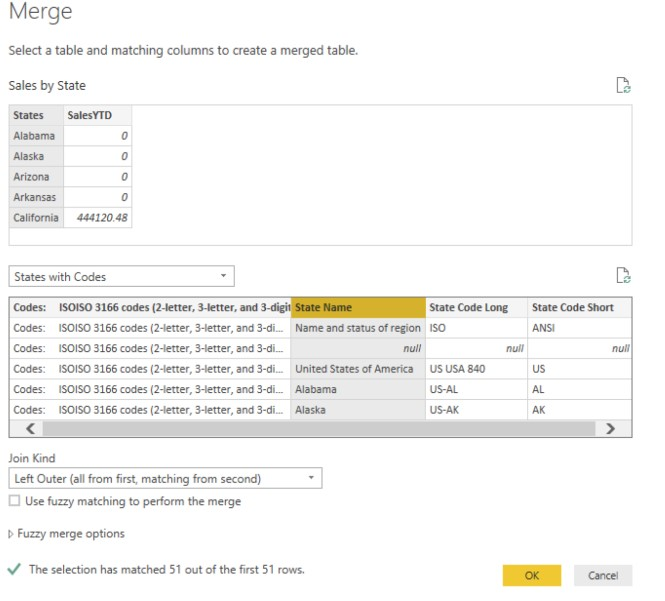
\includegraphics[width=15cm]{./Imagenes/image33} 
	\end{center}
\textbf{ }\\
\textbf{ }\\
\textbf{ }\\
\textbf{ }\\
\textbf{Ejercicio 2: Construyendo Reportes en Power BI}\\
\textbf{ }\\
\textbf{Tarea 1: } Crear un Gráfico\\
\textbf{ }\\
1. En Power BI Desktop, en la barra derecha de navegación, hacer click en Reporte (Report).\\
2. En el panel de Visualizaciones (Visualizations), hacer click en Gauge.\\
3. Arrastar el campo LineTotal de la table Sales a la propiedad Valor (Value) del objeto gauge.\\
4. Arrastrar la medida TargetSales de la table Sales a la propiedad Valor destino (Target value) del objeto
gauge.\\
5. Haga clic en Format, exppandir Gauge axis, y luego en el cuadro Max, escriba 146000.\\
6. Expandir Titulo (Título), en el cuadro Texto de Titulo (Título de texto), tipear Meta de Ventas (Target Sales), y
luego haga clic en Centro.\\
7. Haga clic en el lienzo del informe y luego arrastre el campo CompanyName de la tabla Clientes al informe.
Power BI crea automáticamente una tabla.\\
8. Arrastar el campo LineTotal de la tabla Ventas en el informe.\\
9. Asegúrese de que la tabla tenga el foco y luego, en el panel Visualizaciones, haga clic en Gráfico circular.\\
10. Expanda el gráfico para hacer visibles todos los nombres de las empresas utilizando los controladores de cambio de tamaño en el borde
de la tabla.\\
11. Con el foco aún en el gráfico circular, haga clic en Formato y luego expanda Título.\\
12. En el cuadro Texto del título, escriba Clientes más vendidos y luego haga clic en Centro.\\
13. Arrastar el campo Categoría principal de la tabla Tabla de ventas en el lienzo del informe. Power BI crea una tabla.\\
14. Arrastar el campo OrderQty dentro de la tabla.\\
15. En el panel Visualizaciones, haga clic en Gráfico de barras apiladas.\\
16. En el panel Visualizaciones, haga clic en Campos.\\
17. Arrastre el campo OrderQty a la propiedad de saturación de color. Tenga en cuenta que los colores cambian.\\
18. En el panel Visualizaciones, haga clic en Análisis, expanda Línea constante y luego haga clic en Agregar.\\
19. En el cuadro Valor, escriba 500.\\
20. Cambie el color a rojo, cambie la etiqueta Datos a Activado y luego cambie el color a rojo.\\
21. En el panel Visualizaciones, haga clic en Formato y expanda Título.\\
22. En el cuadro Texto del título, escriba Pedidos por categoría principal y luego haga clic en Centro.\\
23. Haga clic en el lienzo del informe para enfocarlo y luego, en el panel Visualizaciones, haga clic en Gráfico de anillos.\\
24. En la tabla Ventas, seleccione MainCategory y LineTotal.\\
25. En el panel Visualizaciones, haga clic en Formato y luego expanda Título.\\
26. En el cuadro de texto Título, escriba Ventas por categoría principal y luego haga clic en Centro.\\
27. Arrastre el campo Producto de la tabla Ventas al lienzo del informe. Power BI crea una tabla.\\
28. Arrastre el campo LineTotal de la tabla Ventas al gráfico de la tabla de productos.\\
29. En la tabla Ventas, seleccione el campo Categoría principal.\\
30. En el panel Visualizaciones, haga clic en Campos.\\
31. En el panel Filtros, expanda LineTotal (Todos).\\
32. En la lista Mostrar elementos cuando el valor, seleccione es mayor que, y luego en el cuadro a continuación, escriba 32000.\\
33. Hacer clic en Aplicar filtro (Aplicar filtro).\\
34. Expanda MainCategory (All) y luego seleccione Bikes.\\
35. En el panel Visualizaciones, haga clic en Gráfico de columnas apiladas.\\
36. En el panel Visualizaciones, haga clic en Formato y luego expanda Título.\\
37. En el cuadro de texto Título, escriba Las 10 bicicletas más vendidas y luego haga clic en Centro.\\
38. En el panel Visualizaciones, haga clic en Análisis, expanda Línea constante y luego haga clic en Agregar.\\
39. En el cuadro Valor, escriba 35000 y luego configure Color en rojo.\\
40. Cambie la etiqueta de Datos a Activado y luego configure Color en rojo.\\
41. Expanda el gráfico para llenar el espacio restante en el lienzo del informe. Si es necesario, mueva sus imágenes
alrededor para que encajen.\\
42. Haga clic en Guardar.\\

\textbf{ }\\
\begin{center}
	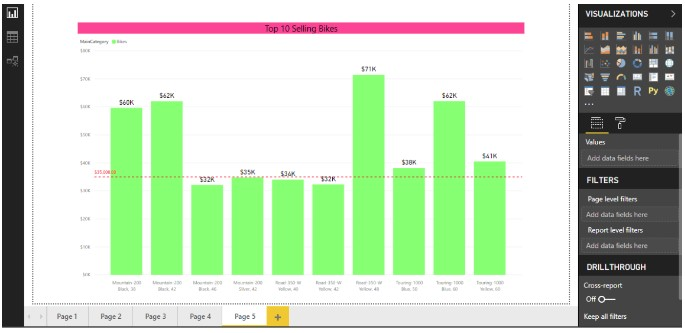
\includegraphics[width=15cm]{./Imagenes/image34} 
	\end{center}
\textbf{ }\\
\textbf{ }\\
\begin{center}
	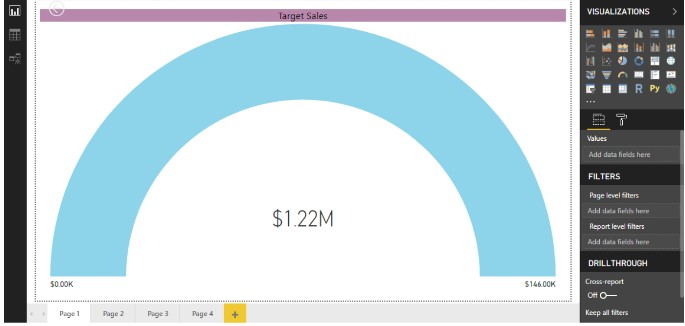
\includegraphics[width=15cm]{./Imagenes/image35} 
	\end{center}
\textbf{ }\\
\textbf{ }\\
\begin{center}
	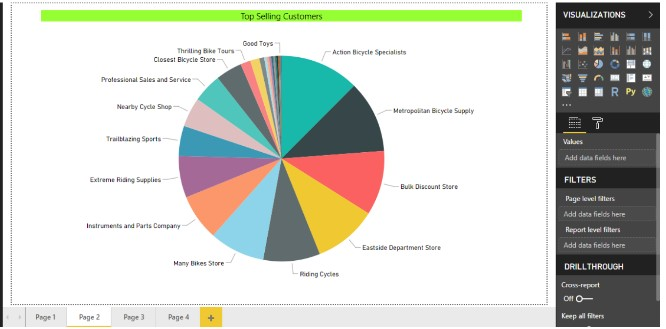
\includegraphics[width=15cm]{./Imagenes/image36} 
	\end{center}
\textbf{ }\\
\textbf{ }\\
\begin{center}
	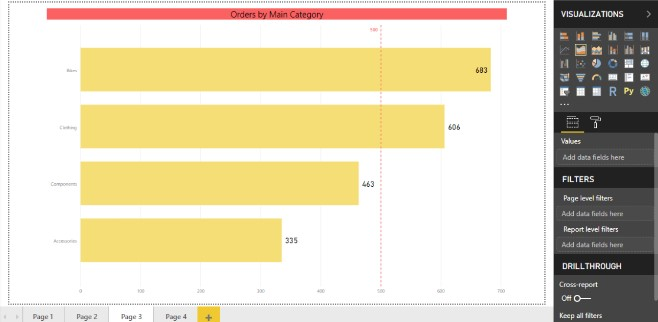
\includegraphics[width=15cm]{./Imagenes/image37} 
	\end{center}
\textbf{ }\\
\textbf{ }\\
\begin{center}
	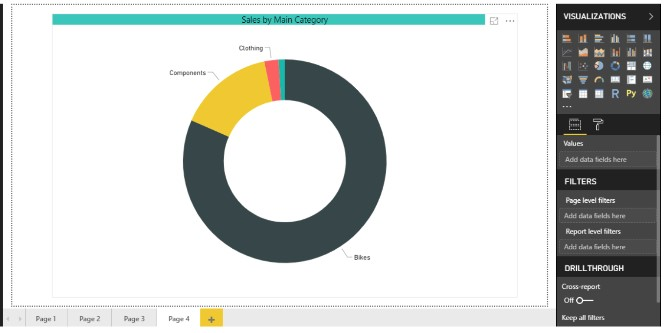
\includegraphics[width=15cm]{./Imagenes/image38} 
	\end{center}
\textbf{ }\\


\textbf{Tarea 2: } Crear una Visualización de Mapa \\
\textbf{ }\\

1. En la parte inferior del informe, haga clic en el ícono + para agregar una nueva página.\\
2. En el panel Campos, en la tabla Clientes, seleccione el campo Ciudad. Power BI agrega un mapa al informe.\\
3. En el panel Campos, en la tabla Ventas, seleccione el campo LineTotal.\\
4. Usando la herramienta de captura en el lado derecho del gráfico, cambie el tamaño del mapa para mostrar todas las burbujas.\\
5. Observe que las burbujas tienen un tamaño proporcional para representar los datos.\\
6. En el panel Visualizaciones, haga clic en Formato y luego expanda Título.\\
7. En el cuadro Texto del título, escriba Ventas mundiales por ciudad y luego haga clic en Centro.\\
8. Haga clic en el lienzo del informe y luego, en la tabla Ventas por estado, seleccione la columna Código de estado. Power BI
agrega automáticamente un mapa.\\
9. En la tabla Ventas por estado, seleccione la columna SalesYTD.\\
10. En el panel Visualizaciones, haga clic en Mapa lleno. Usando la herramienta de captura en el lado derecho y en la parte inferior de
En el gráfico, cambie el tamaño del mapa para mostrar todos los estados.\\
11. Observe que las ventas se agrupan en un área.\\
12. Coloque el cursor en California (CA) para ver la cifra de ventas. El valor no ha sido formateado como moneda.\\
13. En la tabla Ventas por estado, haga clic en la columna SalesYTD.\\
14. En la cinta de Modelado, seleccione Formato: General, haga clic en Moneda y luego seleccione \$ Inglés (United
Fijado).\\
15. Posicione el cursor en California (CA) en el mapa y observe que el valor ha sido formateado.\\
16. En el panel Visualizaciones, haga clic en Formato y luego expanda Título.\\
17. En el cuadro Texto del título, escriba Ventas por estado y luego haga clic en Centro.\\
18. Haga clic en Guardar y luego deje el informe abierto para el próximo ejercicio.\\
Resultados: después de este ejercicio, debería haber creado un informe que tenga gráficos visuales y esté listo para publicar en
El servicio Power BI.\\
\textbf{ }\\
\begin{center}
	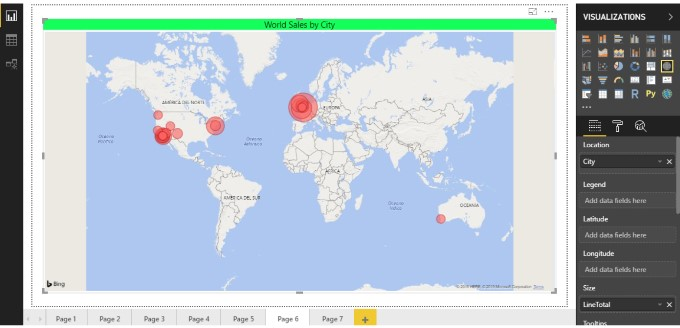
\includegraphics[width=15cm]{./Imagenes/image39} 
	\end{center}
\textbf{ }\\
\textbf{ }\\
\begin{center}
	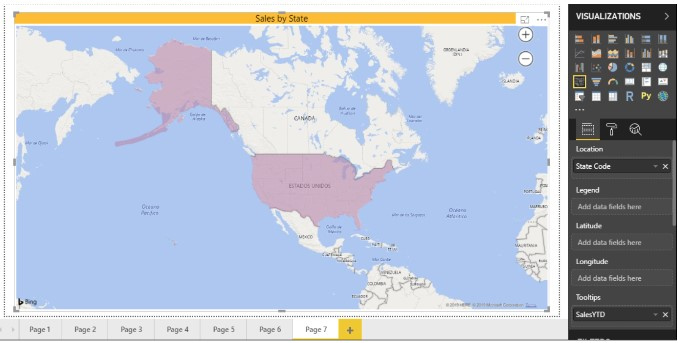
\includegraphics[width=15cm]{./Imagenes/image40} 
	\end{center}
\textbf{ }\\


\end{itemize} 


\end{flushleft}

\end{document}